\documentclass[11pt,letterpaper]{article}

\usepackage{showlabels}
\usepackage{fullpage}
\usepackage{pslatex}
\usepackage[english]{babel}
\usepackage[utf8]{inputenc}
\usepackage{amsmath}
\usepackage{bm}
\usepackage{xcolor}
\usepackage{url}
\usepackage{rotating}
\usepackage{natbib}
\usepackage{amssymb}
\usepackage{lingmacros}


%\usepackage{linguex}
%\usepackage{lingmacros}

\usepackage{CJKutf8}
\newcommand{\korean}[1]{\begin{CJK}{UTF8}{mj}#1\end{CJK}}

\usepackage{tikz}


\usepackage{colortbl}

%\usepackage{xeCJK}

\usepackage{natbib}
\bibliographystyle{unsrtnat}

%\usepackage{latexsym}
\usepackage[english]{babel}
\usepackage[utf8]{inputenc}
\usepackage{bm}
\usepackage{graphicx}
%\usepackage{tikz}
\usepackage{xcolor}
\usepackage{url}
%\usepackage[colorinlistoftodos]{todonotes}
\usepackage{rotating}
\usepackage{multirow}




\usepackage{hyperref}

\usepackage{tikz-dependency}
\usepackage{changepage}
\usepackage{longtable}


\newcommand{\R}[0]{\mathbb{R}}
\newcommand{\Prob}[0]{\mathbb{P}}
\newcommand{\Ff}[0]{\mathcal{F}}

\usepackage{multirow}

\newcommand{\soft}[1]{}
\newcommand{\nopreview}[1]{}
\newcommand\comment[1]{{\color{red}#1}}
\newcommand\michael[1]{{\color{red}(#1)}}
\newcommand\mhahn[1]{{\color{red}(#1)}}
\newcommand\becky[1]{{\color{blue}(#1)}}
\newcommand\note[1]{{\color{red}(#1)}}
\newcommand\jd[1]{{\color{red}(#1)}}
\newcommand\rljf[1]{{\color{red}(#1)}}
\newcommand{\key}[1]{\textbf{#1}}

\DeclareMathOperator*{\argmax}{arg\,max}
\DeclareMathOperator*{\argmin}{arg\,min}
\DeclareMathOperator{\E}{\mathop{\mathbb{E}}}



%\usepackage{lingmacros}
%\usepackage{linguex}


\usepackage{amsthm}

\newcommand{\thetad}[0]{{\theta-d}}
\newcommand{\thetal}[0]{{\theta-{LM}}}

\newcounter{theorem}
\newtheorem{proposition}[theorem]{Proposition}
\newtheorem{thm}[theorem]{Theorem}
\newtheorem{corollary}[theorem]{Corollary}
\newtheorem{question}[theorem]{Question}
\newtheorem{example}[theorem]{Example}
\newtheorem{defin}[theorem]{Definition}
\newtheorem{definition}[theorem]{Definition}
\newtheorem{lemma}[theorem]{Lemma}


%\usepackage{linguex}
%\newcommand{\key}[1]{\textbf{#1}}



\renewcommand{\thefigure}{S\arabic{figure}}
\renewcommand{\thetable}{S\arabic{table}}
\renewcommand{\thesection}{S\arabic{section}}

\newcommand{\utterance}{\mathcal{U}}
\newcommand{\tree}{\mathcal{T}}



\usepackage{siunitx}



\usepackage{longtable}



\frenchspacing
%\def\baselinestretch{0.975}

%\emnlpfinalcopy
%\def\emnlppaperid{496}

\title{Supplementary Information: Morpheme Ordering across Languages reflects optimization for Memory Efficiency}

\begin{document}

\maketitle

\tableofcontents

%\section{Estimating Memory--Surprisal Tradeoffs and Constructing Optimized Orderings}




\section{Identifying Morphemes from Corpus Data}

Here, we describe how we identified morphemes from corpus data and arrived at the classification of morphemes in the six languages as described in the main paper.

%\subsection{General Remarks}
%In order to collect morpheme ordering data, we first need to identify and label morphemes for each language. The Korean, Japanese, and Sesotho corpora have words segmented into the grapheme representations of their morphemes. However, the Turkish, Hungarian, and Finnish corpora do not segment the words into morphemes, but rather include a list of features (such as person, number, voice, etc.) present in each word. We built segmenters to reconstruct the order of morphemes in each word from those feature labels. 

%The Korean corpus came with segmented morphemes labeled with fine-grained categories such as "ending final marker," or "predicative maker," which were the labels we used for the specific morpheme meaning segmenter. We also built a segmenter to take in each segment and output the abstract morpheme slot it fills (such as ``formality"), similar to the abstract slot labelling we did with Turkish, Hungarian, and Finnish. 

%We built two different segmenters for each of the Turkish, Hungarian, and Finnish corpora. One version was ``coarse-grained," meaning that we recovered the order of suffixes in the word on an abstract level, such as a list of ``subject person, subject number." The other version was ``fine-grained," meaning that we used more specific labels for each suffix, such as ``2nd person, plural." In the models, each word is represented as its list of coarse-grained labels, and the model tries to predict the fine-grained labels based on the coarse-grained abstract morphemes. As such, the model tries to order the fine-grained labels, but the surprisal is calculated on the basis of the coarse-grained abstract morphemes.
    
%We built segmenters on two different levels of abstraction for the Finnish, Hungarian, and Turkish corpora. The more fine-grained segmenter version takes the list of morphological features present in a particular word and reconstructs the natural order of morphemes, labelling each morpheme with its specific meaning, such as ``2nd person plural subject." The more abstract segmenter takes the list of morphological features for each word and reconstructs the filled abstract morpheme slots for that word, where each slot has generic label such as ``agreement." For example, in Hungarian, the only possible slots of suffixes appearing after a verb root are voice, mood, tense, agreement, and clitics. As such, we can assign each slot an integer representing the order in which the slots can be filled in a certain language. 

\subsection{Korean Verb Suffixes}

Korean verb morphology is very complex, and there is no generally agreed-upon description in terms of morphemes and slots.
We extracted suffixes based on the annotation found in the corpus we used (Kaist corpus, \citet{chun2018building}) and the linguistic literature on Korean \citep{yeon2010korean}.
The Kaist corpus already provides segmentation into morphemes; we postprocessed it in two ways:
First, we made it more fine-grained by splitting morphemes that are merged in the annotation, and, second, we abstracted away consistently from allomorphy.
For instance, the Kaist corpus separately labels the segments \korean{ㅂ니다} \textit{-mnida} (as in \korean{합니다} \textit{hamnida} `does') and \korean{습니다} \textit{-seumnida} (as in \korean{했습니다} \textit{hatseumnida} `did').
These two segments actually are allomorphs, conditioned by the preceding material.
Furthermore, they can both be segmented into the formal marker \korean{ㅂ/습} (\textit{-p/-seup}, we label this underlying morpheme ``\textsc{p}$_5$'', see below for this notation), and the mood markers \korean{니} (\textit{-ni}, our \textsc{ni}$_6$) and \korean{다} (\textit{-da}, our \textsc{da}$_7$).
We therefore transform both segments into the abstract morpheme sequence \textsc{p}$_5$-\textsc{ni}$_6$-\textsc{da}$_7$ (see below for this notation).
We then partitioned the resulting morphemes into slots that make it possible to consistently describe the ordering of all forms encountered in the corpus.
We indexed morphemes by a small-caps representation of a stylized phonological representation (such as \textsc{p} for -\korean{ㅂ/습}  -\textit{p/seup}),\footnote{These transcriptions are purely conventional, we do not intend these to correspond to a theory of how underlying phonological forms are realized as surface phone strings.} with a subscript indicating their slot (such as \textsc{p}$_5$-\textsc{ni}$_6$-\textsc{da}$_7$).
With this procedure, we identified the nine slots described below:
\begin{enumerate}
    %. The root may include a valency suffix, which is not separated frem the root in the dataset. We did not attempt to separate v
    \item Derivation: The two derivational suffixes are \textit{ha} (\citep[4.1.2]{yeon2010korean}) and the predicative \textit{i}, whose function is similar to that of a copula \citep[4.1.4]{yeon2010korean}.
    
    \item Honorific \textsc{si}$_3$ \citep[4.3.2, 4.4.1]{yeon2010korean}
    \item Tense/Aspect suffixes include -\textsc{ess}$_4$ for past \citep[4.5.1.1]{yeon2010korean}, -\textsc{essess}$_4$ for remote past \citep[4.5.1.2]{yeon2010korean}, -\textsc{get}$_4$ for future \citep[4.5.2.1]{yeon2010korean}
    \item Formality \textsc{p}$_5$ (allomorphs include -\textit{p}-, -\textit{m}-, -\textit{seum}-,  \citep[4.3.2]{yeon2010korean})
    \item Mood 1: We partition Mood suffixes into two slots, as these can be combined into strings of combined mood suffixes. Frequent elements of the Mood I slot are -\textsc{n}$_6$-, -\textsc{ni}$_6$- \citep[4.3.2]{yeon2010korean}.
    
    \item Mood II: Frequent elements of the Mood II slot are declarative -\textsc{da}$_7$- \citep[4.3.2]{yeon2010korean}, command -\textsc{ra}-, interrogative -\textsc{ka}-, the suffix  -\textsc{ji} \citep[4.2.2-3]{yeon2010korean}, and informal -\textsc{eo}$_7$-.
    
    \item Polite -yo
    \item Conjunctive endings, such as -go, -seo,  and others
    
\end{enumerate}

We show morphemes occurring at least 50 times in slots 2-8 in Figure~\ref{tab:korean-frequent-morphemes}.
We do not provide the list of the (very numerous) conjunctive and nominalizing suffixes as these are not the focus of the typological generalization that we are interested in.

Additional morphemes that occur less than 50 times are placed into an UNKNOWN slot, this affects \textcolor{red}{TODO} \% of morpheme occurrences in the dataset.


%TODO 
%- Yeon 4.4.2.2 kkeo object honorific % 꺼   % does not seem to appear in Kaist corpus?


%Frequent morphemes:
\begin{table}
\resizebox{1\textwidth}{!}{
\begin{tabular}{llllllllll}
Slot & Morphs & Short & Description & Citation \\ \hline\hline
Derivation & \korean{하} & \textsc{ha}$_2$ &	  & \citep[4.1.2]{yeon2010korean}\\
& \korean{이} & \textsc{i}$_2$ &	 & \citep[4.1.4]{yeon2010korean} \\ \hline
Honorific & \korean{시} 	& \textsc{si}$_3$ & &\citep[4.3.2, 4.4.1]{yeon2010korean}\\\hline
	Tense/Asp. & \korean{었었} 	& \textsc{essess}$_4$ &  & \citep[4.5.1.2]{yeon2010korean} \\
&\korean{겠} 	& \textsc{get}$_4$ & assertive & \citep[4.5.2.1]{yeon2010korean}\\
& \korean{ㅆ} &\textsc{ess}$_4$ & past& \citep[4.5.1.1]{yeon2010korean}\\\hline
Formality & \korean{ㅂ} &\textsc{p}$_5$ &	 formal-polite &\citep[4.3.2]{yeon2010korean}\\\hline
	Mood 1& \korean{리} & \textsc{ri}$_6$ &	 \\ % I-guess-
	&\korean{니} 	&\textsc{ni}$_6$ & See Table~\ref{tab:korean-hada-1} & \citep[4.3.2]{yeon2010korean}\\
	&\korean{ㄴ} 	&\textsc{n}$_6$ &See Table~\ref{tab:korean-hada-1}  \\\hline
	Mood 2& \korean{시다} & \textsc{sida}$_7$ & 	Hortative, formal, polite \\
       & \korean{어} 	& \textsc{eo}$_7$ & Indicative, informal\\
	& \korean{자} & \textsc{ja}$_7$&	 Hortative & \citep[4.3.6.3]{yeon2010korean}\\
	& \korean{소} &\textsc{so}$_7$  &	See Table~\ref{tab:korean-styles} \\
	& \korean{ㄹ까} & \textsc{lkka}$_7$& Interrogative & \citep[8.9]{yeon2010korean} \\
	& \korean{오} & \textsc{o}$_7$  & See Table~\ref{tab:korean-styles} \\
	& \korean{지} & \textsc{ji}$_7$ &	    & \citep[4.2.2-3]{yeon2010korean}\\
	& \korean{까} 	& \textsc{ka}$_7$ & Interrogative & \citep[4.3.4, p. 175; p. 183]{yeon2010korean} \\
	& \korean{라} &\textsc{ra}$_7$  &	 command & \citep[4.3.6.4]{yeon2010korean} \\
	& \korean{다} & \textsc{da}$_7$ &	 Declarative & \citep[4.3.2]{yeon2010korean} &  \\\hline
	Polite & \korean{요} & \textsc{yo}$_8$&	 See Table~\ref{tab:korean-styles} \\
\end{tabular}
}
\caption{Frequent Korean verb suffixes in slots 1-8. The first column describes the nine slots. Second column: Representation of one allomorph in Hangeul. Third column: Identifier.}\label{tab:korean-frequent-morphemes}
\end{table}


Next, we explain how our segmentation corresponds to commonly described paradigms.
First, in Table~\ref{tab:korean-styles}, we describe the correspondence to the speech style system described by \citep[4.3.2]{yeon2010korean}.
Second, in Tables~\ref{tab:korean-hada-1}--\ref{tab:korean-hada-3}, we show the paradigm for the verb \korean{하다} \textit{hada} `to do' as described in Wiktionary.\footnote{ \texttt{https://en.wiktionary.org/wiki/\korean{하다}} (retrieved Septemgber 16, 2020).}
In Table~\ref{tab:kroean-itda}, we show the part of the paradigm of the verb \textit{ida} `to be' corresponding to Table~\ref{tab:korean-hada-1} (the other parts of the paradigm are analogous to those of \textit{hada}).
Note that none of these paradigms constitute exhaustive lists of all forms of these verbs; instead, they represent commonly used forms in a systematic paradigmatic representation.


\begin{table}
	\begin{center}
\begin{tabular}{l||l|l|l|llll}
            & Statement & Question  & Command    & Proposal    \\ \hline\hline
Formal      &  \korean{ㅂ니다} & \korean{ㅂ니까} & \korean{지-ㅂ-지오} & \korean{지-ㅂ-지다} \\ 
      &  -mnida & -mnikka  & -sipsio & -sipsida  \\ 
      &  -\textsc{p}$_5$-\textsc{ni}$_6$-\textsc{da}$_7$ & -\textsc{p}$_5$-\textsc{ni}$_6$-\textsc{kka}$_7$  & -\textsc{si}$_3$-\textsc{p}$_5$-\textsc{sio}$_7$ & -\textsc{si}$_3$-\textsc{p}$_5$-\textsc{sida}$_7$ \\ \hline
Polite      &  \multicolumn{4}{c}{\korean{아/어/요}}  \\
      &  \multicolumn{4}{c}{-a/eoyo}  \\
            & \multicolumn{4}{c}{-\textsc{eo}$_7$-\textsc{yo}$_8$} \\ \hline
Semi-Formal & \korean{오/소}   &           &   \korean{오}       &  \korean{-ㅂ-지다} \\
&  -o/so   &           & -o        & -p-sida \\
	&  -\textsc{o}$_7$/-\textsc{so}$_7$   &           & -\textsc{o}$_7$    & -\textsc{p}$_5$-\textsc{sida}$_7$ \\\hline
Familiar    &    \korean{네}    &  \korean{나/는가} &  \korean{게}      &    \korean{세} \\
            & -ne                  & -na/neunka & -ge & -se \\ 
	    & -\textsc{ne}$_7$                  & -\textsc{na}$_7$/-\textsc{neunka}$_7$ & -\textsc{ge}$_9$ & \textsc{-se}$_9$ \\ \hline
Intimate      &  \multicolumn{4}{c}{\korean{아/어}}  \\
      &  \multicolumn{4}{c}{-a/eo}  \\
            & \multicolumn{4}{c}{-\textsc{eo}$_7$} \\ \hline
Plain       &   \korean{다}     &  \korean{(느)냐} &  \korean{라}     &  \korean{자}\\
            &  -da    &  -(neu)nya & -ra      & -ja \\
	    & -\textsc{da}$_7$    &   -\textsc{nya}$_7$          & -\textsc{ra}$_7$      & -\textsc{ja}$_7$\\
\end{tabular}
	\end{center}
\caption{Correspondence between our morpheme segmentation and the speech style system described by \citep[4.3.2]{yeon2010korean}. In each cell, we provide the Hangul ending given by \citep{yeon2010korean}, a transliteration, and a representation in terms of underlying morphemes.}\label{tab:korean-styles}
\end{table}



\begin{table}
\begin{tabular}{llllllllll}
           &          &Formal non-polite & Informal non-polite & Informal polite & Formal polite \\ \hline \hline
\multirow{6}{*}{Indicative} & \multirow{3}{*}{Non-past} & \korean{한다} & \korean{해}  & \korean{해요}  & \korean{합니다}  \\
           &          & handa & hae & haeyo &  hamnida \\
           &          & -\textsc{n}$_6$-\textsc{da}$_7$ & -\textsc{eo}$_7$ & -\textsc{eo}$_7$-\textsc{yo}$_8$ &  -\textsc{p}$_5$-\textsc{ni}$_6$-\textsc{da}$_7$ \\
           &          & \korean{하+ㄴ다}  & \korean{하+어}    & \korean{하+어+요} & \korean{하+ㅂ니다} \\
            &          &  px+ef        &   pvg+ecs        & pvg+ef+jxf & pvg+ef\\
           \hline
           & \multirow{3}{*}{Past}     & \korean{했다}  & \korean{했어} & \korean{했어요}   & \korean{했습니다}  \\
           &      & haet-da &  haesseo &  haesseoyo  & haetseumnida \\
           &      & -\textsc{ess}$_4$-\textsc{da}$_7$ &  -\textsc{ess}$_4$-\textsc{eo}$_7$ &  -\textsc{ess}$_4$-\textsc{eo}$_7$-\textsc{yo}$_8$  & -\textsc{ess}$_4$-\textsc{p}$_5$-\textsc{ni}$_6$-\textsc{da}$_7$ \\
           &      &  \korean{하+었+다}  &  \korean{하+었+어} & \korean{하+었+어+요} & \korean{하+었+습니다}  \\
           &      &  ncpa+xsv+ep+ef   & px+ep+ef   &   px+ep+ef+jxf &     pvg+ep+ef\\
           \hline
\multirow{6}{*}{Interrogative} & \multirow{3}{*}{Non-past} & \korean{하느냐} & \korean{해}  & \korean{해요}  & \korean{합니까} \\
 &  & haneunya &  hae &  haeyo & hamnikka\\
 &  & -\textsc{nya}$_7$ &  -\textsc{eo}$_7$ &  -\textsc{eo}$_7$-\textsc{yo}$_8$ & -\textsc{p}$_5$-\textsc{ni}$_6$+KKA$_7$ \\
               && \korean{하+느냐} & & & \korean{하+ㅂ니까}    \\
              && px+ef & & & px+ef \\
 \hline
              & \multirow{3}{*}{Past} & \korean{했느냐} & \korean{했어} & \korean{했어요} & \korean{했습니까} \\
              &  & ha-n-neunya &  hae-sseo &  hae-sseo-yo &  haetseumnikka\\
              &  & -\textsc{ess}$_4$-\textsc{nya}$_7$ &  -\textsc{ess}$_4$-\textsc{eo}$_7$ &  -\textsc{ess}$_4$-\textsc{eo}$_7$+YO$_8$ &  -\textsc{ess}$_4$-\textsc{p}$_5$-\textsc{ni}$_6$-\textsc{kka}$_7$\\
              &  &  \korean{하+었+느냐}  & \korean{하+었+어} & \korean{하+었+어+요} & \korean{하+었+습니까} \\
              &  & +ep+ef  & +ep+ef            & px+ep+ef+jxf & pvg+ep+ef \\
              \hline
Hortative   && \korean{하자}  & \korean{해}  & \korean{해요}  & \korean{합시다}  \\
   && haja &  hae &  haeyo & hapsida \\
   && -JA$_7$ &  -\textsc{eo}$_7$ &  -\textsc{eo}$_7$-\textsc{yo}$_8$ & -\textsc{p}$_5$-\textsc{sida}$_7$ \\
   && \korean{+자} && \korean{하+어+요} & \korean{하+ㅂ시다}\\
   && +ef  && pvg+ef+jxf & ef \\
   \hline
Imperative  && \korean{해라, 하여라}  & \korean{해}  & \korean{해요}  & \korean{합시오}  \\
  && haera, hayeora &  hae &  haeyo &  hapsio \\
  && -\textsc{ra}$_7$ & -\textsc{eo}$_7$ & -\textsc{eo}$_7$-\textsc{yo}$_8$ & -\textsc{p}$_5$-\textsc{si}$_3$O \\
  && \korean{하+어라}, \korean{하+어라}  &  &    & \korean{+ㅂ시오} \\
  && pvg+ef,  pvg+ef                     &  &    &  +ef\\
  \hline
Assertive   && \korean{하겠다}  & \korean{하겠어}  & \korean{하겠어요}  & \korean{하겠습니다}  \\
   &&  hagetda & hagesseo &  hagesseoyo & hagetseumnida \\
   &&  -\textsc{get}$_4$-\textsc{da}$_7$ & -\textsc{get}$_4$-\textsc{eo}$_7$ &  -\textsc{get}$_4$-\textsc{eo}$_7$-\textsc{yo}$_8$ & \textsc{get}$_4$-\textsc{p}$_5$-\textsc{ni}$_6$-\textsc{da}$_7$ \\
&& \korean{하+겠+다}  & \korean{하+겠+어}   & \korean{하+겠+어+요} & \korean{하+겠+습니다}\\
&&  px+ep+ef          & pvg+ep+ef   & pvg+ep+ef+jxf & pvg+ep+ef\\
\hline
\end{tabular}
	\caption{Correspondence between our morpheme segmentation and the paradigm of \textit{hada} `to do' as described by Wiktionary and in the Kaist treebank. In each cell, we provide the Hangul  and transliterated (e.g., handa) forms given by Wiktionary, a representation in terms of underlying morphemes (e.g., -\textsc{n}$_6$-\textsc{da}$_7$), and -- where available -- how the form is segmented in the Kaist corpus (e.g., px+ef).}\label{tab:korean-hada-1} % (e.g., \korean{한다})\korean{하+ㄴ다} and 
\end{table}

\begin{table}
	\begin{center}
\begin{tabular}{llllllllll}
           &          &Formal non-polite & Informal non-polite & Informal polite & Formal polite \\ \hline \hline
Cause/Reason && \korean{해} & \korean{해서, 하여서} & \korean{하니} & \korean{하니까} \\
&& hae & haeseo, hayeoseo & hani & hanikka \\ 
&& -\textsc{eo}$_7$ & -\textsc{eoseo}$_9$ & -\textsc{ni}$_9$ & -\textsc{nikka}$_9$ \\
&& &\korean{하+어서, 하+어서} & \korean{하+니} & \korean{하+니까} \\
&& & pvg+ecs, xsm+ecs         & pvg+ecs & xsm+ef \\
\hline
Contrast && \korean{하지만} & \korean{하는데} & \korean{하더니} \\
 && hajiman & haneunde & haedoni & \\ 
 && -\textsc{jiman}$_9$ & -\textsc{neunde}$_9$ & -\textsc{deoni}$_9$ & \\ \hline
Conjunction && \korean{하고} \\
 && hago \\ 
	&& -\textsc{go}$_9$ \\ \hline
Condition && \korean{하면} & \korean{해야, 하여야} \\
&& hamyeon & haeya, hayeoya \\
	&& -\textsc{meyon}$_9$ & -\textsc{eoya}$_9$ \\ \hline
Motive && \korean{하려고} \\
 && haryeogo \\
	&& -\textsc{ryeogo}$_9$
\end{tabular}
	\end{center}
	\caption{Continuation of Table~\ref{tab:korean-hada-1}: Forms of \textit{hada} with a conjunctive ending.}\label{tab:korean-hada-2}
\end{table}



\begin{table}[]
    \centering
    \begin{tabular}{llllllllllllllllllllllllll}
           &          &Formal non-polite & Informal non-polite & Informal polite & Formal polite \\ \hline \hline
\multirow{2}{*}{Indicative} & Non-past & \korean{하신다} & \korean{하셔} & \korean{하세요, 하셔요} & \korean{하십니다} \\
                           && -\textsc{si}$_3$-\textsc{n}$_6$-\textsc{da}$_7$ & \textsc{si}$_3$-\textsc{eo}$_7$ & \textsc{si}$_3$-\textsc{eo}$_7$-\textsc{yo} & \textsc{si}$_3$-\textsc{p}$_5$-\textsc{ni}$_6$-\textsc{da}$_7$ \\
&& \korean{하+시+ㄴ다}       &   --   &    \korean{하+시+어+요}             &  \korean{하+시+ㅂ니다}        \\
\hline
&& \korean{하셨다} & \korean{하셨어} & \korean{하셨어요} & \korean{하셨습니다} \\
&& \textsc{si}$_3$-\textsc{ess}$_4$-\textsc{da}$_7$ & \textsc{si}$_3$-\textsc{ess}$_4$-\textsc{eo}$_7$ & \textsc{si}$_3$-\textsc{ess}$_4$-\textsc{eo}$_7$-\textsc{yo} & \textsc{si}$_3$-\textsc{ess}$_4$-\textsc{p}$_5$-\textsc{ni}$_6$-\textsc{da}$_7$ \\
& & \korean{하+셨+다}       &  --    &        --        &  \korean{하+셨+습니다}       \\
\hline
\multirow{2}{*}{Interrogative} & Non-past & \korean{하시느냐} & \korean{하셔} & \korean{하세요, 하셔요} & \korean{하십니까} \\
&& \textsc{si}$_3$-\textsc{nya}$_7$ & \textsc{si}$_3$-\textsc{eo}$_7$ & \textsc{si}$_3$-\textsc{eo}$_7$-\textsc{yo} & \textsc{si}$_3$-\textsc{p}$_5$-\textsc{ni}$_6$-\textsc{kka}$_7$ \\
& &   --     &   --   &   \korean{하+시+어+요}             &  --        \\
\hline
& Past & \korean{하셨느냐} & \korean{하셨어} & \korean{하셨어요} & \korean{하셨습니까} \\
&      & \textsc{si}$_3$-\textsc{ess}$_4$-\textsc{nya}$_7$ & \textsc{si}$_3$-\textsc{ess}$_4$-\textsc{eo}$_7$          & \textsc{si}$_3$-\textsc{ess}$_4$-\textsc{eo}$_7$-\textsc{yo} & \textsc{si}$_3$-\textsc{ess}$_4$-\textsc{p}$_5$-\textsc{ni}$_6$-\textsc{kka}$_7$ \\
& &        &      &                &          \\
\hline
\multirow{2}{*}{Imperative} && \korean{하시라} & \korean{하셔} & \korean{하세요} & \korean{하십시오} \\
&& -\textsc{si}$_3$-RA & -\textsc{si}$_3$-\textsc{eo}$_7$ & -\textsc{si}$_3$-\textsc{eo}$_7$-\textsc{yo} & -\textsc{si}$_3$-\textsc{p}$_5$-\textsc{si}$_3$O \\
&        &      & \korean{하+시+어+}               &   \korean{하+십시오}       \\
\hline
\multirow{2}{*}{Assertive} & & \korean{하시겠다} & \korean{하시겠어} & \korean{하시겠어요} & \korean{하시겠습니다} \\
&        &  -\textsc{si}$_3$-\textsc{get}$_4$-\textsc{da}$_7$     &  -\textsc{si}$_3$-\textsc{get}$_4$-\textsc{eo}$_7$              &  -\textsc{si}$_3$-\textsc{get}$_4$-\textsc{eo}$_7$-\textsc{yo} & -\textsc{si}$_3$-\textsc{get}$_4$-\textsc{p}$_5$-\textsc{ni}$_6$-\textsc{da}$_7$        \\
&& -- & -- & -- & -- \\
    \end{tabular}
    \caption{Continuation of Tables~\ref{tab:korean-hada-1}--\ref{tab:korean-hada-2}: Conjugation of hada with an honorific (\textsc{si}$_3$). We provide Hangul forms, morpheme sequences, and -- where available -- segmentations as given in the Kaist corpus.}
    \label{tab:korean-hada-3}
\end{table}

%itda \url{https://en.wiktionary.org/wiki/%EC%9E%88%EB%8B%A4#Korean}

\begin{table}[]
    \centering
    \begin{tabular}{llllllllllllllllllllllllllllllllll}
           &          &Formal non-polite & Informal non-polite & Informal polite & Formal polite \\ \hline \hline
    \multirow{6}{*}{Indicative}         & Non-past  & \korean{있다} & \korean{있어} & \korean{있어요} & \korean{있습니다} \\
         &  &  \korean{있+다} & \korean{있+어} & \korean{있+어+요} & \korean{있+습니다}\\
         &  &  -\textsc{da}$_7$            & -\textsc{eo}$_7$            & -\textsc{eo}$_7$-\textsc{yo}            & -\textsc{p}$_5$-\textsc{ni}$_6$-\textsc{da}$_7$ \\
         &  & +ef & +ef & +ef+jxf & +ef \\
         \hline
 & Past & \korean{있었다} & \korean{있었어} & \korean{있었어요} & \korean{있었습니다} \\
         &  & \korean{있+었+다} & \korean{있+었+어} & \korean{있+었+어+요} & \korean{있+었+습니다}\\
         && -\textsc{ess}$_4$-\textsc{da}$_7$            & \textsc{ess}$_4$-\textsc{eo}$_7$             & \textsc{ess}$_4$-\textsc{eo}$_7$-\textsc{yo} & -\textsc{ess}$_4$-\textsc{p}$_5$-\textsc{ni}$_6$-\textsc{da}$_7$ \\
         &  & +ep+ef & +ep+ef & +ep+ef+jxf & +ep+ef \\
         \hline
\multirow{6}{*}{Interrogative} & Non-past  & \korean{있느냐} & \korean{있어} & \korean{있어요} & \korean{있습니까} \\
&& -\textsc{nya}$_7$ & -\textsc{eo}$_7$ & -\textsc{eo}$_7$-\textsc{yo} & -\textsc{p}$_5$-\textsc{ni}$_6$-\textsc{kka}$_7$ \\
         &  & \korean{있+느냐} & \korean{있+어} & \korean{있+어+요} & \korean{있+습니까}\\
         &  & +ef              & +ef  & +ef+jxf & +ef\\
         \hline
         & Past & \korean{있었느냐} & \korean{있었어} & \korean{있었어요} & \korean{있었습니까} \\
         && -\textsc{ess}$_4$-\textsc{nya}$_7$ & -\textsc{ess}$_4$-\textsc{eo}$_7$ & -\textsc{ess}$_4$-\textsc{eo}$_7$-\textsc{yo} & -\textsc{ess}$_4$-\textsc{p}$_5$-\textsc{ni}$_6$-\textsc{kka}$_7$ \\
         &  & \korean{있+었+느냐} & \korean{있+었+어} & \korean{있+었+어+요}\\
         &  & +ep+ef & paa+ep+ef &  paa+ep+ef+jxf\\
         \hline
\multirow{3}{*}{Assertive} &  & \korean{있겠다} & \korean{있겠어} & \korean{있겠어요} & \korean{있겠습니다} \\
&& -\textsc{get}$_4$-\textsc{da}$_7$ & -\textsc{get}$_4$-\textsc{eo}$_7$ & -\textsc{get}$_4$-\textsc{eo}$_7$-\textsc{yo} & -\textsc{get}$_4$-\textsc{p}$_5$-\textsc{ni}$_6$-\textsc{da}$_7$ \\
         &  & \korean{있+겠+다} & \korean{} & \korean{있+겠+어+요} & \korean{있+겠+습니다}\\
         &  & +ep+f             &           & paa+ep+ef+jxf & paa+ep+ef\\
    \end{tabular}
    \caption{Conjugation of \textit{itda}. Refer to Table~\ref{tab:korean-hada-1} for details.}
    \label{tab:kroean-itda}
\end{table}



%\begin{longtable}{lllll}
%NOMINALIZER-future-determiner-\korean{을} & EUL &	 128 \\
%NOMINALIZER-topic?past-determiner-\korean{은} & EUN&	 129 \\
%NOMINALIZER-nominalizer-informal-nonpolite-gi & GI &	 151 \\
%NOMINALIZER-nominalizer-formal-nonpolite-m 	& M & 216 \\
%\end{longtable}





\subsection{Finnish Verb Inflection}

In the Finnish corpus, verb forms are annotated using collections of features, such as \texttt{Mood=Ind} and \texttt{Number=Sing}, which make it pssible to uniquely map the form to a cell of the paradigm in Table~\ref{tab:finnish} \footnote{From \url{https://en.wiktionary.org/wiki/tulla\#Conjugation}, retrieved January 10, 2021.}.

\begin{table}
\begin{tabular}{l|llllll}
	TAM & Agreement & Form & Suffixes \\ \hline\hline
	present tense & 	1st sing& 	tulen  & -n$_{\textsc{Agr}}$\\ 
	\cite[Section 24]{karlsson1999finnish}	&	2nd sing. 	& 	tulet  & -t$_{\textsc{Agr}}$\\ 
	&	3rd sing. 	& 	tulee  & -V$_{\textsc{Agr}}$\\                
	&	1st plur. 	& 	tulemme  &-mme$_{\textsc{Agr}}$\\ 
	&	2nd plur. 	& 	tulette  &-tte$_{\textsc{Agr}}$\\ 
	&	3rd plur. 	& 	tulevat  &-vat$_{\textsc{Agr}}$\\ 
	&	passive 	& 	tullaan  &-t$_{\textsc{Passive}}$-Vn$_{\textsc{Agr}}$ \\  \hline
past tense 	 	&	1st sing.& 	tulin & -i$_{\textsc{TAM}}$-n$_{\textsc{Agr}}$\\  
	Karlsson section 60&	2nd sing. &	tulit  & -i$_{\textsc{TAM}}$-t$_{\textsc{Agr}}$\\ 
	&	3rd sing. &	tuli  & -i$_{\textsc{TAM}}$-V$_{\textsc{Agr}}$\\ 
	&	1st plur. &	tulimme  &-i$_{\textsc{TAM}}$-mme$_{\textsc{Agr}}$\\ 
	&	2nd plur. &	tulitte  &-i$_{\textsc{TAM}}$-tte$_{\textsc{Agr}}$\\ 
	&3rd plur. &	tulivat  & -i$_{\textsc{TAM}}$-vat$_{\textsc{Agr}}$\\ 
	&	passive &	tultiin  &-t$_{\textsc{Passive}}$-i$_{\textsc{TAM}}$-Vn$_{\textsc{Agr}}$ \\  \hline
conditional mood  &1st sing. &	tulisin  & -isi$_{\textsc{TAM}}$-n$_{\textsc{Agr}}$\\ 
	(-isi-, \cite[Section 65]{karlsson1999finnish})	&2nd sing. &	tulisit  & -isi$_{\textsc{TAM}}$-t$_{\textsc{Agr}}$\\ 
	&3rd sing. &	tulisi  & -isi$_{\textsc{TAM}}$-V$_{\textsc{Agr}}$\\ 
	&1st plur. &	tulisimme  & -isi$_{\textsc{TAM}}$-mme$_{\textsc{Agr}}$\\ 
	&2nd plur. &	tulisitte  & -isi$_{\textsc{TAM}}$-tte$_{\textsc{Agr}}$\\ 
	&3rd plur. &	tulisivat  & -isi$_{\textsc{TAM}}$-vat$_{\textsc{Agr}}$ \\ 
	&passive &	tultaisiin  & -ta$_{\textsc{Passive}}$-isi$_{\textsc{TAM}}$-Vn$_{\textsc{Agr}}$\\  \hline
	imperative mood  &1st sing. &	-- \\ 
	 \cite[Section 66]{karlsson1999finnish}	 & 2nd sing. &	tule & - \\ 
	&	3rd sing. &	tulkoon  & -kV$_{\textsc{TAM}}$-oon$_{\textsc{Agr}}$\\ 
	&	1st plur. &	tulkaamme  & -kV$_{\textsc{TAM}}$-mme$_{\textsc{Agr}}$\\ 
	&	2nd plur. &	tulkaa   & -kV$_{\textsc{TAM}}$\\ 
	&	3rd plur. 	&tulkoot  & -kV$_{\textsc{TAM}}$-vat$_{\textsc{Agr}}$\\ 
	&	passive 	&tultakoon  & -ta$_{\textsc{Passive}}$-kV$_{\textsc{TAM}}$-Vn$_{\textsc{Agr}}$\\ \hline
	potential mood 	 &	1st sing. &	tullen  & -ne$_{\textsc{TAM}}$-n$_{\textsc{Agr}}$\\ 
		(-ne-, \cite[Section 67]{karlsson1999finnish}) & 2nd sing. &	tullet  & -ne$_{\textsc{TAM}}$-t$_{\textsc{Agr}}$\\ 
	&	3rd sing. &	tullee  & -ne$_{\textsc{TAM}}$-V$_{\textsc{Agr}}$\\ 
	&	1st plur. &	tullemme  & -ne$_{\textsc{TAM}}$-mme$_{\textsc{Agr}}$\\ 
	&	2nd plur. &	tullette  & -ne$_{\textsc{TAM}}$-tte$_{\textsc{Agr}}$\\ 
	&	3rd plur. &	tullevat  & -ne$_{\textsc{TAM}}$-vat$_{\textsc{Agr}}$\\ 
	&	passive &	tultaneen  & -t$_{\textsc{Passive}}$-ne$_{\textsc{TAM}}$-Vn$_{\textsc{Agr}}$ \\ \hline
\end{tabular}
	\caption{Finnish verb inflection}\label{tab:finnish}
\end{table}

\subsection{Turkish Verb Suffixes}

In Table~\ref{tab:turkish-suffixes}, we show the list of identified Turkish verb suffixes.
In Figure~\ref{tab:turkish-yapmak}, we show how our segmentation corresponds to the paradigm of \textit{yapmak} as described by Wiktionary.\footnote{From https://en.wiktionary.org/wiki/yapmak\#Turkish, retrieved September 5, 2020.}



\begin{table}
\resizebox{\textwidth}{!}{
\begin{tabular}{ll||lll|lllllllllll}
         &        & 1 sg.      & 2   sg.     & 3  sg.      & 1  pl.    & 2 pl.     & 3 pl. \\ \hline\hline
 DNP & A & yaparım & yaparsın &  	yapar & yaparız & yaparsınız &  	yaparlar \\
                    &  & -\textsc{ar}$_5$-\textsc{im}$_8$ & -\textsc{ar}$_5$-\textsc{sin}$_8$ &  	-\textsc{ar}$_5$ & -\textsc{ar}$_5$-\textsc{iz}$_8$ & -\textsc{ar}$_5$-\textsc{siniz}$_8$ &  	-\textsc{ar}$_5$-\textsc{lar}$_6$ \\ \hline
                & I & yapıyorum & yapıyorsun & 	yapıyor &	yapıyoruz &	yapıyorsunuz &	yapıyorlar \\
		&  & -\textsc{iyor}$_5$-\textsc{im}$_8$ & -\textsc{iyor}$_5$-\textsc{sin}$_8$ & 	-\textsc{iyor}$_5$ &	-\textsc{iyor}$_5$-\textsc{iz}$_8$ &	-\textsc{iyor}$_5$-\textsc{siniz}$_8$ &	-\textsc{iyor}$_5$-\textsc{lar}$_6$ \\ \hline
                & Pr  & yapacağım &	yapacaksın 	& yapacak 	& yapacağız &	yapacaksınız &	yapacaklar \\ 
                &   & -\textsc{acak}$_5$-\textsc{im}$_8$ &	-\textsc{acak}$_5$-\textsc{sin}$_8$ 	& -\textsc{acak}$_5$ 	& -\textsc{acak}$_5$-\textsc{iz}$_8$ &	-\textsc{acak}$_5$-\textsc{siniz}$_8$ &	-\textsc{acak}$_5$-\textsc{lar}$_6$ \\ \hline\hline
        DP    & Pe &yaptım &	yaptın &	yaptı &	yaptık &	yaptınız &	yaptılar \\
	      &  &-\textsc{ti}$_5$-\textsc{im}$_8$ &	-\textsc{ti}$_5$-\textsc{sin}$_8$ &	-\textsc{ti}$_5$ &	-\textsc{ti}$_5$-\textsc{k}$_8$ &	-\textsc{ti}$_5$-\textsc{siniz}$_8$ &	-\textsc{ti}$_5$-\textsc{lar}$_6$ \\ \hline
                & I & yapıyordum &	yapıyordun &	yapıyordu &	yapıyorduk &	yapıyordunuz &	yapıyorlardı \\ 
		&  & -\textsc{iyor}$_5$-\textsc{du}$_7$-\textsc{im}$_8$ &	-\textsc{iyor}$_5$-\textsc{du}$_7$-\textsc{sin}$_8$ &	-\textsc{iyor}$_5$-\textsc{du}$_7$ &	-\textsc{iyor}$_5$-\textsc{du}$_7$-\textsc{k}$_8$ &	-\textsc{iyor}$_5$-\textsc{du}$_7$-\textsc{siniz}$_8$ &	-\textsc{iyor}$_5$-\textsc{lar}$_6$-\textsc{du}$_7$ \\ \hline\hline
 I     & Pe & yapmışım &	yapmışsın &	yapmış &	yapmışız &	yapmışsınız &	yapmışlar \\
       &  & -\textsc{mis}$_5$-\textsc{im}$_8$ &	-\textsc{mis}$_5$-\textsc{sin}$_8$ &	-\textsc{mis}$_5$ &	-\textsc{mis}$_5$-\textsc{iz}$_8$ &	-\textsc{mis}$_5$-\textsc{siniz}$_8$ &	-\textsc{mis}$_5$-\textsc{lar}$_6$ \\ \hline
               & A & yaparmışım &	yaparmışsın &	yaparmış &	yaparmışız &	yaparmışsınız& 	yaparlarmış \\ 
            &  & -\textsc{ar}$_5$-\textsc{mis}$_7$-\textsc{im}$_8$ &	-\textsc{ar}$_5$-\textsc{mis}$_7$-\textsc{sin}$_8$ &	-\textsc{ar}$_5$-\textsc{mis}$_7$ &	-\textsc{ar}$_5$-\textsc{mis}$_7$-\textsc{iz}$_8$ &	-\textsc{ar}$_5$-\textsc{mis}$_7$-\textsc{siniz}$_8$& 	-\textsc{ar}$_5$-\textsc{lar}$_6$-\textsc{mis}$_7$ \\ \hline
               & I & yapıyormuşum &	yapıyormuşsun &	yapıyormuş &	yapıyormuşuz &	yapıyormuşsunuz &	yapıyorlarmuş \\
	       &              & -\textsc{iyor}$_5$-\textsc{mis}$_7$-\textsc{im}$_8$ &	-\textsc{iyor}$_5$-\textsc{mis}$_7$-\textsc{sin}$_8$ &	-\textsc{iyor}$_5$-\textsc{mis}$_7$ &	-\textsc{iyor}$_5$-\textsc{mis}$_7$-\textsc{iz}$_8$ &	-\textsc{iyor}$_5$-\textsc{mis}$_7$-\textsc{sunuz}$_8$ &	-\textsc{iyor}$_5$-\textsc{lar}$_6$-\textsc{mis}$_7$ \\
\end{tabular}
}
\caption{Paradigm of the Turkish verb \textit{yapmak}. This paradigm covers TAM and agreement suffixes.}\label{tab:turkish-yapmak}
\end{table}

\begin{table}
\begin{tabular}{llllllll}
Slot & Label & Function & Morphs & Reference \\ \hline
\hline
	Valence & -TIR$_1$  & Causative & -tIr & \\
\hline
	Voice &  -IL$_2$ & Passive & -Il\\
%\hline
%Polite &   & \\
\hline
Polarity  & MA$_3$ & Negation & -mA \\
\hline
Mood  & EBIL$_4$ & Abilitative & -Ebil & \cite{schaaik2020turkish}, section 21 \\
      & IN$_4$   & Imperative & -In & \cite{schaaik2020turkish}, section 18.1 \\
\hline
TAM1      & AR$_5$ & Aorist, nonpast, direct & -(I/E)r, -z  & \cite{schaaik2020turkish}, section 20.5 (`Present-2') \\
          & IYOR$_5$ & Imperfective, direct & -Iyor \\
          & ACAK$_5$ & Prospective, nopast, direct & -AcAk & \cite{schaaik2020turkish}, section 20.2\\
          & MIS1$_5$  & Perfective, indirect & -mIş & \cite{schaaik2020turkish}, section 20.3\\
          & TI$_5$ & Perfective, past, direct & -dI & \cite{schaaik2020turkish}, section 20.4\\
%\hline
%V Noun &  \\
\hline
	3rd Plural& \textsc{lar}$_{6}$  & 3rd Plural & -lAr & \\
\hline
TAM2      & MUS2$_7$ & Aorist/Imperfective, indirect & -mIş & \cite{schaaik2020turkish}, section 24.2 \\
          & DU$_7$ & imperfective, past, direct & -dI & \cite{schaaik2020turkish}, section 24.1.3 \\
\hline
	Agreement & IM$_8$ & 1st singular & -Im\\
	  & SIN$_8$ &2nd singular & -sIn\\
	  & IZ$_8$  & 1st plural & -Iz\\
	  & SINIZ$_8$ & 2nd plural & -sInIz \\
	  & K$_8$     & 1st plural, past direct & -k\\
%\hline
%Poss Num/Pers & \\
\hline
\end{tabular}
	\caption{Verb suffixes in Turkish, arranged by slot. The first column describes slots as in the main paper. The second column lists the unique identifiers for each morpheme. The third column describes the function and meaning; the fourth column describes the approximate phonological form (see \citet[Section 5.1]{schaaik2020turkish} for the vowels I, A, E).}\label{tab:turkish-suffixes}
\end{table}




\subsection{Hungarian Verb Suffixes}


In Table~\ref{tab:hungarian-suffixes}, we show the list of identified Hungarian verb suffixes.
In Figure~\ref{tab:hungarian-paradigms}, we show how our segmentation corresponds to the paradigm of three verbs as described by Wiktionary.\footnote{From \texttt{https://en.wiktionary.org/wiki/tesz},
\texttt{https://en.wiktionary.org/wiki/csinál},
\texttt{https://en.wiktionary.org/wiki/ismer}, retrieved September 5, 2020.}





\begin{table}
    \centering
    \begin{tabular}{lllllllll}
    Slot & Morpheme & Function & Reference    \\ \hline\hline
Valence	    & AT$_1$ & Causative &   \cite{rounds2001hungarian} 4.5.3 \\ \hline
Mood	    & HET$_2$ & Potential &   \cite{rounds2001hungarian} 4.5.1  \\
         & N$_2$ & conditional &   \cite{rounds2001hungarian} 4.3.7 \\
         & J$_2$ & subjunctive &   \cite{rounds2001hungarian} 4.3.5 \\
\hline
	    Tense& T$_3$ & indicative past &  \cite{rounds2001hungarian} 4.3.3 \\
         \hline
Finiteness  & NI$_4$ & Infinitive  &  \cite{rounds2001hungarian} 4.4.4 \\
\hline
%Definiteness & I & definite 2/3pl \\
%         \hline
Agreement (Obj+Subj)         & & See Table~\ref{tab:hungarian-paradigms} & \cite{rounds2001hungarian} 4.3 \\
%         & EL$_5$ & 2sg present\\
%         & UNK$_5$ & 1pl present\\
%         & TEK$_5$& 2pl\\
%         & NEK$_5$ & 3pl present\\
%         & EM$_5$ & 1sg past or definite \\
%         & ED$_5$ & 2sg definite \\
         \hline
    \end{tabular}
    \caption{Hungarian verb suffixes}
    \label{tab:hungarian-suffixes}
\end{table}

\begin{table}[]
    \centering
\resizebox{\textwidth}{!}{
    \begin{tabular}{lll||lll|lll|llllllllll}
	    &&& \multicolumn{3}{c|}{Singular} & \multicolumn{3}{c}{Plural} & \cite{rounds2001hungarian} \\
    &    & &  1 & 2 & 3 & 1 & 2 & 3 \\ \hline
Ind & Pres   &  I    & teszek &	teszel &	tesz &	teszünk &	tesztek &	tesznek \\
    &        &       & csinálok &	csinálsz &	csinál &	csinálunk &	csináltok &	csinálnak \\
   &&&  ismerek &	ismersz &	ismer &	ismerünk &	ismertek &	ismernek \\
 &    &      & -ek & -sz & -- & -{\"u}nk & -tek & -nek &  4.3.1.1\\
 &    &      & -\textsc{ek}$_{\textsc{Agr}}$ &	-\textsc{el}$_{\textsc{Agr}}$ &	-- &	-\textsc{unk}$_{\textsc{Agr}}$ &	-\textsc{tek}$_{\textsc{Agr}}$ &	-\textsc{nek}$_{\textsc{Agr}}$  \\
	    \hline
   &&  D    & teszem &	teszed &	teszi &	tesszük &	teszitek &	teszik \\
   &&       & csinálom &	csinálod &	csinálja &	csináljuk &	csináljátok &	csinálják \\
  &&& ismerem &	ismered &	ismeri &ismerjük &	ismeritek &	ismerik \\
    &&      & -em & -ed & -i & -j{\"u}k & -itek & -ik &  4.3.1.2\\
 && & -\textsc{em}$_{\textsc{Agr}}$ &	-\textsc{ed}$_{\textsc{Agr}}$ &	-\textsc{i}$_{\textsc{Agr}}$ &	-\textsc{iuk}$_{\textsc{Agr}}$ &	-\textsc{itek}$_{\textsc{Agr}}$ &	-\textsc{ik}$_{\textsc{Agr}}$  \\ 
	    \hline
%   && 2po      & teszlek \\ 
%	    &&& -lek \\
%	    \hline\hline
& Past &     I    &tettem &	tettél &	tett &	tettünk &	tettetek &	tettek \\
&      &          & csináltam &	csináltál &	csinált &	csináltunk &	csináltatok &	csináltak \\
&&&ismertem &	ismertél &	ismert &	ismertünk &	ismertetek &	ismertek \\
	    &  &        &-t-em & -t-{\'e}l & -t & -t-{\"u}nk & -t-etek & -t-ek &   4.3.3.1\\
	    &  &         &-\textsc{t}$_{\textsc{Tense}}$-\textsc{em}$_{\textsc{Agr}}$ &	-\textsc{t}$_{\textsc{Tense}}$-\textsc{eel}$_{\textsc{Agr}}$ &	-\textsc{t}$_{\textsc{Agr}}$ &	-\textsc{t}$_{\textsc{Tense}}$-\textsc{unk}$_{\textsc{Agr}}$ &	-\textsc{t}$_{\textsc{Tense}}$-\textsc{etek}$_{\textsc{Agr}}$ &	-\textsc{t}$_{\textsc{Tense}}$-\textsc{ek}$_{\textsc{Agr}}$ &\\ 
	    \hline
 & &   D    &tettem &	tetted &	tette &	tettük &	tettétek &	tették \\
 & &        & csináltam &	csináltad &	csinálta &	csináltuk &	csináltátok &	csinálták \\
&&& ismertem &	ismerted &	ismerte &	ismertük &	ismertétek 	&ismerték \\
	    &  &      & -t-em & -t-ed & -t-e & -t-{\"u}k & -t-{\'e}tek & -t-{\'e}k &   4.3.3.2 \\
	    & &       &-\textsc{t}$_{\textsc{Tense}}$-\textsc{em}$_{\textsc{Agr}}$ &	-\textsc{t}$_{\textsc{Tense}}$-\textsc{ed}$_{\textsc{Agr}}$ &	-\textsc{t}$_{\textsc{Tense}}$-\textsc{i}$_{\textsc{Agr}}$ &	-\textsc{t}$_{\textsc{Tense}}$-\textsc{uk}$_{\textsc{Agr}}$ &	-\textsc{t}$_{\textsc{Tense}}$-\textsc{eetek}$_{\textsc{Agr}}$ &	-\textsc{t}$_{\textsc{Tense}}$-\textsc{eek}$_{\textsc{Agr}}$  & \\ 
	    \hline
%  &&       &tettelek  & (\cite{rounds2001hungarian} 4.3.3.2) \\ 
%	    &&       & -\textsc{t}$_{	extsc{Tense}}$-\textsc{elek} \\
%  \hline
Cond  &Pres &   I    &tennék &	tennél &	tenne &	tennénk &	tennétek &	tennének \\
      &     &        & csinálnék &	csinálnál &	csinálna &	csinálnánk 	&csinálnátok &	csinálnának \\
  &&&    ismernék &	ismernél &	ismerne &	ismernénk &	ismernétek &	ismernének \\
  &&& -n{\'e}k & -n{\'e}l & -ne & -n{\'e}nk & -n{\'e}tek & -n{\'e}nek &  4.3.7.1\\
	    & &   I    &-\textsc{ne}$_{\textsc{Mood}}$-\textsc{ek} &	-\textsc{ne}$_{\textsc{Mood}}$-\textsc{el} &	-\textsc{ne}$_{\textsc{Mood}}$ &	-\textsc{ne}$_{\textsc{Mood}}$-\textsc{enk} &	-\textsc{ne}$_{\textsc{Mood}}$-\textsc{etek} &	-\textsc{ne}$_{\textsc{Mood}}$-\textsc{enek}  \\
  \hline
   &&  D    &tenném &	tennéd &	tenné &	tennénk &	tennétek &	tennék \\
   &&       & csinálnám &	csinálnád &	csinálná &	csinálnánk &	csinálnátok &	csinálnák \\
 &&&  ismerném &	ismernéd &	ismerné &	ismernénk 	&ismernétek &	ismernék \\
&&&     -n{\'e}m & -n{\'e}d & -n{\'e} & -n{\'e}nk & -n{\'e}tek & -n{\'e}k &   4.3.7.2\\ 
	    &&      &-\textsc{ne}$_{\textsc{Mood}}$-\textsc{em}$_{\textsc{Agr}}$ &	-\textsc{ne}$_{\textsc{Mood}}$-\textsc{ed}$_{\textsc{Agr}}$ &	-\textsc{ne}$_{\textsc{Mood}}$-\textsc{e}$_{\textsc{Agr}}$ &	-\textsc{ne}$_{\textsc{Mood}}$-\textsc{enk}$_{\textsc{Agr}}$ &	-\textsc{ne}$_{\textsc{Mood}}$-\textsc{etek}$_{\textsc{Agr}}$ &	-\textsc{ne}$_{\textsc{Mood}}$-\textsc{ek}$_{\textsc{Agr}}$  \\
	    \hline
%	    && -n{\'e}lek  \\
%	    && -\textsc{ne}-\textsc{lek} \\
 %      &&  &tennélek \\ \hline
Subj & Pres & I         &tegyek &	tégy or tegyél &	tegyen &	tegyünk &	tegyetek &	tegyenek \\
     &      &           & csináljak &	csinálj or
csináljál &	csináljon &	csináljunk& 	csináljatok &	csináljanak \\
&&&ismerjek &	ismerj or
ismerjél &	ismerjen &	ismerjünk &	ismerjetek &	ismerjenek \\
 & &          & -j-ek & -j-({\'e}l) & -j-en & -j-{\"u}nk & -j-etek & -j-enek  &  4.3.5.1\\
	    &  &          &-\textsc{j}$_{\textsc{Mood}}$-\textsc{ek} &	\textsc{j}$_{\textsc{Mood}}$-\textsc{eel} &	-\textsc{j}$_{\textsc{Mood}}$-\textsc{en} &	-\textsc{j}$_{\textsc{Mood}}$-\textsc{unk} &	-\textsc{j}$_{\textsc{Mood}}$-\textsc{etek} &	-\textsc{j}$_{\textsc{Mood}}$-\textsc{enek}\\
 \hline
&&D         &tegyem &	tedd or tegyed &	tegye &	tegyük& 	tegyétek &	tegyék \\
&&          & csináljam &	csináld or
csináljad &	csinálja &	csináljuk &	csináljátok &	csinálják \\
&&&ismerjem &	ismerd or
ismerjed &	ismerje &	ismerjük &	ismerjétek & ismerjék
 \\
  &&       & -j-em & -j-ed & -j-e & -j-{\"u}k & -j-{\'e}tek & -j-{\'e}k &  4.3.5.2\\
&&         &-\textsc{j}$_{\textsc{Mood}}$-\textsc{em}$_{\textsc{Agr}}$ &	-\textsc{j}$_{\textsc{Mood}}$-\textsc{ed}$_{\textsc{Agr}}$ &	-\textsc{j}$_{\textsc{Mood}}$-\textsc{e}$_{\textsc{Agr}}$ &	-\textsc{j}$_{\textsc{Mood}}$-\textsc{uk}$_{\textsc{Agr}}$ & 	-\textsc{j}$_{\textsc{Mood}}$-\textsc{eetek}$_{\textsc{Agr}}$ &	-\textsc{j}$_{\textsc{Mood}}$-\textsc{eek}$_{\textsc{Agr}}$\\ 
	    \hline
 % &&       &tegyelek & (\cite{rounds2001hungarian} 4.3.5.2)\\
%	    &&& \textsc{j}-\textsc{elek} \\
    \end{tabular}
    }
    \caption{Hungarian verb suffixes: Inflection by tense, mood, definitiness, and person/number. ``Ind'' = ``Indicative'', ``Cond'' = ``Conditional'', ``Subj'' = ``Subjunctive'', ``I'' = ``Indefinite'', ``D'' = ``Definite''.
    For each form, we show the orthographic shape for three verbs, the suffix as identified by \citet{rounds2001hungarian}, and our representation as a string of morphemes as described in Table~\ref{tab:hungarian-suffixes}.}
    \label{tab:hungarian-paradigms}
\end{table}


\subsection{Sesotho}

We describe Sesotho verb affixes following \cite{Hahn2020modeling}.
who described these based on \citep{doke1967textbook, guma1971outline, demuth1992acquisition}.
We refer to \cite{Hahn2020modeling} for further details.

\begin{enumerate}
    \item Subject agreement: This morpheme encodes agreement with the subject, for person, number, and noun class (the latter only in the 3rd person) \cite[\textsection 395]{doke1967textbook}.
            The annotation provided by \cite{demuth1992acquisition} distinguishes between ordinary subject agreement prefixes and agreement prefixes used in relative clauses; we distinguish these morpheme types here.

    \item Negation \citep[\textsection 429]{doke1967textbook}

    \item Tense/aspect marker   \citep[\textsection 400--424]{doke1967textbook}

    \item Object agreement or reflexive marker \citep[\textsection 459]{doke1967textbook}.
    Similar to subject agreement, object agreement denotes person, number, and noun class features of the object.
\end{enumerate}
We identified the following suffixes:

\begin{enumerate}
\item Semantic derivation: reversive (e.g., `do' $\rightarrow$ `undo')
\item Valence: (e.g., causative, neuter/stative, applicative, and reciprocal)
    \item Voice: passive
    \item Tense
    \item Mood
    \item Interrogative and relative markers
\end{enumerate}

\subsection{Japanese}

%\paragraph{Japanese Verbs}
We describe Japanese verb suffixes following \citep{Hahn2020modeling}, who described these based on \citep{kaiser2013japanese,hasegawa2014japanese}.
We refer to \citep{Hahn2020modeling} for details.

\begin{enumerate}
\item \textit{suru}: obligatory suffix after Sino-Japanese words when they are used as verbs
\item Valence: causative (-\textit{ase}-)
\item Voice and Mood: passive (-\textit{are}-, -\textit{rare}-) and potential (-\textit{e}-, -\textit{are}-, -\textit{rare}-)
\item Politeness (-\textit{mas}-)
\item Mood: desiderative (-\textit{ta}-)
\item Negation (-\textit{n}-)
\item Tense, Aspect, Mood, and Finiteness: past (-\textit{ta}), future/hortative (-\textit{yoo}) \citep[229]{kaiser2013japanese}, nonfiniteness (-\textit{te})
\end{enumerate}


\subsection{Nouns in Finnish. Hungarian, and Turkish}

We illustrate noun suffixes using examples taken from the corpora, with the annotation given in UD and our segmentation, in Table~\ref{tab:noun-affixes-examples}.
In addition to these three slots, Hungarian also has possessed suffixes, marked with \texttt{Number[psed]} in the data.
However, this is rare in the data, occurring only three times in the training set, and was thus excluded.

\begin{table}[]
    \centering
\begin{tabular}{lllllllll}
\multirow{5}{*}{\textsc{Finnish}} & Form & \textit{juttuihisi} \\
 & Lemma & \textit{juttu} \\
& Annotation & \texttt{Case=Ill|Number=Plur|Number[psor]=Sing|Person[psor]=2} \\
& Segmentation & -\textsc{i}-\textsc{hi}-\textsc{si} \\
& Gloss & Stem-Plural-Illative-2SgPoss \\
\hline
\multirow{5}{*}{\textsc{Hungarian}} & Form & \textit{érveiket} \\
& Lemma & \textit{érv}  \\
& Annotation &	\texttt{Case=Acc|Number=Plur|Number[psor]=Plur|Person[psor]=3} \\
& Segmentation & -\textsc{ei}-\textsc{k}-\textsc{et} \\
& Gloss & -Plural-Possessor3rdPlur-Accusative \\
\hline
\multirow{5}{*}{\textsc{Turkish}} & Form & \textit{hareketlerimden} \\
& Lemma & \textit{hareket} \\
& Annotation & 	\texttt{Case=Abl|Number=Plur|Number[psor]=Sing|Person=3|Person[psor]=1}	\\
& Segmentation & -\textsc{lar}-\textsc{im}-\textsc{den} \\
& Gloss & Plural-1sgPoss-Ablative\\
\end{tabular}
    \caption{Noun affixes in Finnish, Hungarian, and Turkish.}
    \label{tab:noun-affixes-examples}
\end{table}



% https://en.wiktionary.org/wiki/h%C3%A1z#Hungarian
%Re Hungarian: Possessed suffixes are very rare, occurring only three times in the training partition. 

%\begin{tabular}{lllllllllllll}
%országokéhoz & ország &	Case=All|Number=Plur|Number[psed]=Sing|Number[psor]=None|Person[psor]=None \\
%-ok-é-hoz \\
%-Plural-PossessedSingular-Allative \\
%országokéhoz &	ország&	Case=All|Number=Plur|Number[psed]=Sing|Number[psor]=None|Person[psor]=None	\\
%kancellárénál&	kancellár &	Case=Ade|Number=Sing|Number[psed]=Sing \\
%lapunkat &	lap &	Case=Acc|Number=Sing|Number[psed]=None|Number[psor]=Plur|Person[psor]=1	\\
%unk-at \\
%érveiket	& érv &	Case=Acc|Number=Plur|Number[psed]=None|Number[psor]=Plur|Person[psor]=3 \\
%ei-k-et \\
%-Plural-Possessor3rdPlur-Accusative \\
%\end{tabular}


%\section{Controlling for Vowel Harmony}\label{sec:vowel-harmony}
%%\subsection{Vowel Harmony in Turkish}
%
%%\url{https://turkishexplained.com/vh1.htm}
%
%We represent words as sequences of abstract morphemes.
%In many languages, morphemes are subject to morphophonological changes depending on the other morphemes that they occur with, which means that morphemes can be expressed as different phoneme sequences depending on the environment.
%Such changes could be taken into account by explicitly distinguishing between different phonological expressions of the same morpheme.
%In most cases, such morphophonological processes only affect neighboring morphemes, but sometimes they involve interactions between non-adjacent morphemes.
%We asked whether our findings about the efficiency of verb suffix ordering continues to hold when explicitly account for morphophonological interactions between non-adjacent morphemes.
%
%Among the languages in our sample, this is instantiated most extensively by Turkish vowel harmony.
%Turkish vowel harmony can largely be described in terms of two underlying vowels ``A'' and ``I'' whose realization depends on the last preceding vowel, as follows:
%
%\begin{center}
%    \begin{tabular}{l|llllll}
%        Preceding & A & I \\ \hline
%        a, I & a & I \\
%        e, i & e & i \\
%        o, u & a & u \\
%        {\"o}, {\"u} & e & {\"u}
%    \end{tabular}
%\end{center}
%
%For most suffixes, vowel harmony can be encoded in terms of one underlying form (see Table~\ref{tab:turkish-suffixes}).
%The suffix AR$_6$ has the form ``Ar'' after most monosyllabic stems, and ``Ir'' after multisyllabic stems or one of 13 exceptional monosyllabic stems.
%
%Vowel harmony can create dependencies between non-adjacent morphemes because the vowel of one morpheme can determine the vowels of multiple subsequent morphemes containing the vowels A or I.
%
%We asked whether our findings about the efficiency of verb suffix ordering continues to hold when explicitly account for vowel harmony.
%That is, we applied the same rules for vowel harmony to hypothetical affix orderings, and encoded realizations of the same morpheme differently when they are assigned different vowels.
%We repeated the same experiments as in the main paper, (i) comparing the AUC to other orderings, and (ii) comparing the optimized and real orderings.
%Results are shown in Figure~\ref{fig:turkish-harmony-results}.
%
%Real orderings have a lower AUC than almost all alternative orderings even when taking vowel harmony into account.
%Furthermore, optimized orderings recover the real orderings with high accuracy both in the ordering of the slots and in predicting orders for forms in the dataset \mhahn{TODO result}.
%
%
\section{Other Measures of Accuracy}

Here we report results using two alternative measures of accuracy.
\textsc{FullAccuracy} measures the fraction of forms in the corpus that are ordered entirely correctly (Figure~\ref{tab:optimized_acc_verbs_full}).
\textsc{FullTypeAccuracy} modifies this by disregarding repeated occurrences of the same form in the corpus (Figure~\ref{tab:optimized_acc_verbs_full_types}).
Results across these two measures and the one reported in the main paper strongly agree both numerically and in the qualitative patterns of the comparison between optimized orderings and baselines.

%
%
%
\begin{figure}[]
    \centering
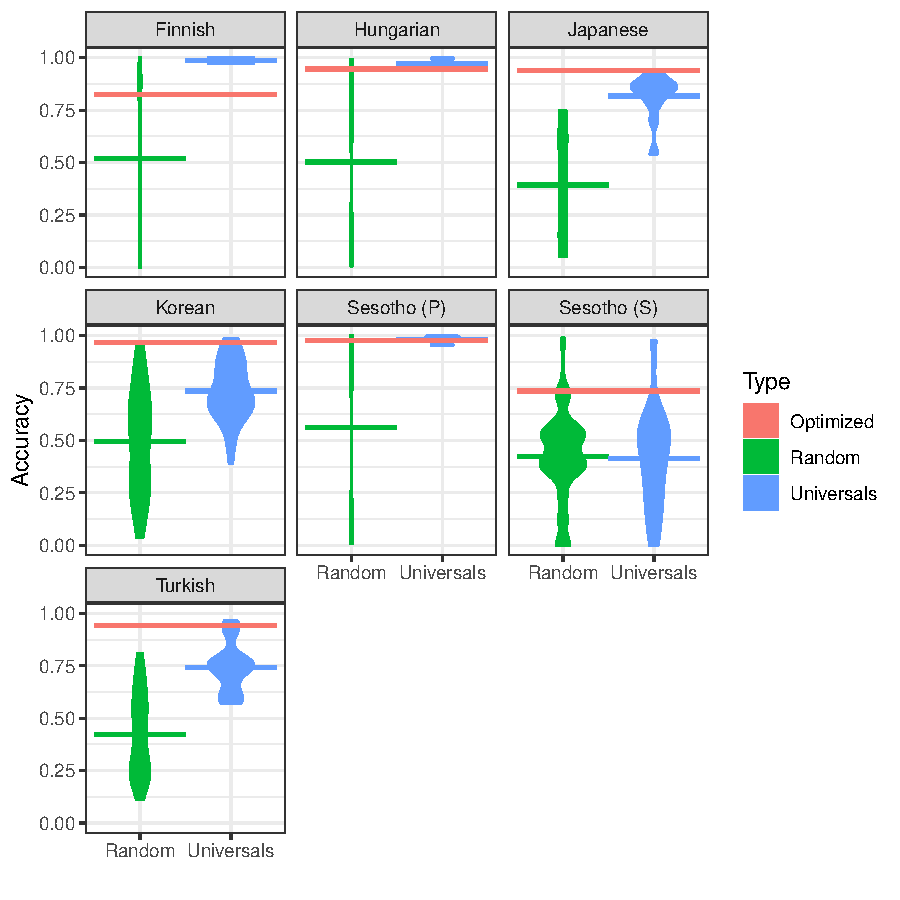
\includegraphics[width=0.8\textwidth]{figures/accuracies_verbs_full.pdf}
    \caption{Accuracies in predicting verb morpheme ordering, according to the \textsc{FullAccuracy} measure.
    For the baselines, we provide both a smoothed violin plot of the distribution of accuracies, and the mean accuracy as a horizontal line (green and blue). For the optimized order, we show the accuracy as a horizontal line (red).
    In all languages, optimized orderings provide higher accuracy than the mean of the random baselines at $p<0.001$.}
    \label{tab:optimized_acc_verbs_full}
\end{figure}
%
\begin{figure}[]
    \centering
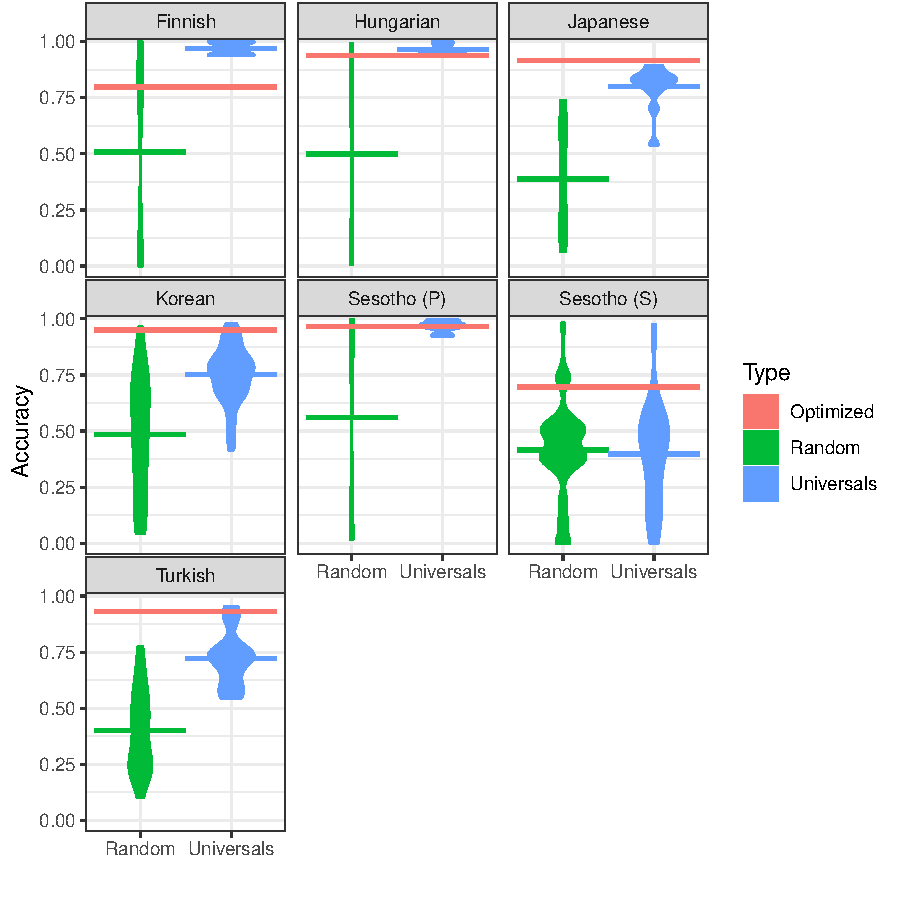
\includegraphics[width=0.8\textwidth]{figures/accuracies_verbs_full_types.pdf}
    \caption{Accuracies in predicting verb morpheme ordering, according to the \textsc{FullTypeAccuracy} measure.
    For the baselines, we provide both a smoothed violin plot of the distribution of accuracies, and the mean accuracy as a horizontal line (green and blue). For the optimized order, we show the accuracy as a horizontal line (red).
    In all languages, optimized orderings provide higher accuracy than the mean of the random baselines at $p<0.001$.}
    \label{tab:optimized_acc_verbs_full_types}
\end{figure}
%




%\section{Other Models}
%
%
%\subsection{Scope-Based Ordering}
%
%
%
%\subsection{Complexity-Based Ordering}
%
%\subsection{Inkelas 2016}
%
%Drawing on the notion of informativity defined by \citet{priva2017informativity}, \citet{inkelas2016affix} considered the informativity between a suffix $S_i$ and the preceding $S_{i-1}$ as
%\begin{equation}
%    \sum_{S_{i-1}, S_{i}} \frac{P(S_{i-1} , S_i)}{P(S_i)} \log P(S_i | S_{i-1})
%\end{equation}
%%They tested this idea in a pilot study of Turkish, finding preliminary evidence that high-informativity suffixes are closer to the root.
%This notion of informativity is similar to $I_1$, only differing in whether the $P(S_i)$ term occurs inside the logarithm:
%\begin{equation}
%   I_1 = \sum_{S_{i-1}, S_{i}} P(S_{i-1} , S_i) \log \frac{P(S_i | S_{i-1})}{P(S_i)}
%\end{equation}
%

\bibliography{literature}
\bibliographystyle{natbib}

\end{document}









\paragraph{Turkish Nouns}
\begin{enumerate}
    \item Number
    \item Possessor number and possessor person
    \item Case 
\end{enumerate}

\paragraph{Hungarian Nouns}
\url{https://cl.lingfil.uu.se/~bea/publ/megyesi-hungarian.pdf}
\begin{enumerate}
    \item Number
    \item Possessor person
    \item Possessor number \becky{Missing in citation}
    \item Case 
\end{enumerate}

\paragraph{Finnish Nouns}
\begin{enumerate}
    \item Derivation
    \item Number
    \item Case 
    \item Possessor person and possessor number
\end{enumerate}


\paragraph{Hungarian Verbs} \url{https://cl.lingfil.uu.se/~bea/publ/megyesi-hungarian.pdf}
\begin{enumerate}
    \item Voice \becky{Missing in citation}
    \item Mood
    \item Tense \mhahn{Potential mood appears in front of Tense, so I changed from Tense--Mood to Mood -- Tense as the order here.}
    \item Definiteness, person, and number: This suffix indicates the definiteness or indefiniteness of the direct object of the verb, as well as the person and number of the subject performing the verb. 
\end{enumerate}

\paragraph{Turkish Verbs}
\begin{enumerate}
    \item Voice
    \item Negation / polarity
    \item Aspect
    \item Evidential 
    \item Tense 
    \item Mood 
    \item Person and Number
    \item Formality
\end{enumerate}

\mhahn{I've changed this to the following}
\begin{enumerate}
    \item Valence (Causative -tir-)
    \item Voice (Passive -il-)
    \item Negation / polarity (Negation -ma-)
    \item Mood (Potential -bil-)
    \item TAM1: Tense, Aspect, Mood, Evidential
    \item 3rd Plural (-lar-)
    \item TAM2: Tense, Aspect, Mood, Evidential
    \item Subject agreement (incorporating TAM information)
    \item Formality (polite -makta-)
    \item Genitive (-dir-)
    \item Verbal Noun (-mak)
    \item Possessive agreement
\end{enumerate}




\paragraph{Finnish Verbs}
\begin{enumerate}
    \item Voice
    \item Tense 
    \item Mood 
    \item Person and number
    \item Clitic
\end{enumerate}


